\pdfoutput=1
\pdfmapfile{+cm.map}
\documentclass{llncs}
\usepackage{graphicx,booktabs,amsmath,amssymb,placeins}
\usepackage[hidelinks]{hyperref}
\pdfinfoomitdate=1
\pdftrailerid{}
\hypersetup{pdftitle={Preference-Robust Screening and Decision Support for Solar-Access Interventions in Urban Renewal},pdfauthor={},pdfcreator={LaTeX}}
\newcommand{\ind}{\mathbf{1}}
\newcommand{\aidraft}{\footnote{AI-assisted preparation~\cite{openai2026}; scope is stated in the AI Use Disclosure.}}
\setlength{\emergencystretch}{2em}
\renewcommand{\textbullet}{\ensuremath{\bullet}}
\renewcommand{\textperiodcentered}{\ensuremath{\cdot}}
\begin{document}
\title{Preference-Robust Screening and Decision Support for Solar-Access Interventions in Urban Renewal}
\author{}\institute{}\maketitle\renewcommand{\thefootnote}{\arabic{footnote}}
\begin{abstract}
An architect assessing solar-access interventions needs alternatives that remain useful before priorities are agreed. A fixed weighted top ten can hide this dependence. We study 630 two-building height-reduction rules in a canonical urban block and replace reliance on one declared score with preference-space analysis and a ten-candidate regret-based shortlist. Newly low-sun area is zero throughout this rule universe, leaving three discriminating criteria: low-sun-area reduction, mean direct-sun gain and nominal removed volume. A frozen protocol uses three preference spaces, each with 20,000 training, test and replication weights. A greedy sampled-minimax heuristic is evaluated independently and checked by continuous linear-programming audits. On the full-simplex test, mean absolute utility regret falls from 0.010759 for the historical top ten to 0.000054; winner coverage rises from 77.695\% to 97.940\%. Continuous worst-case regret falls from 0.246359 to 0.007656. Both sets already have zero regret in the solar-access-priority and local spaces, and the new set recovers fewer members of preference-specific top tens in every space. Five candidates change; three new shortlist members lack archived Honeybee review. Historical simulation and geometry evidence remains separate from these new preference experiments. The contribution is a reproducible, evidence-linked application of established multicriteria and regret ideas to architectural screening, not a new general optimization algorithm or an architect-validated preference model. AI assistance is disclosed~\cite{openai2026}.
\keywords{Decision support \and Preference robustness \and Solar access \and Multicriteria analysis \and Urban renewal}
\end{abstract}

\section{Introduction}
Which interventions should an architect examine when the relative importance of sunlight improvement and building removal has not yet been agreed?\aidraft{} A numerical ranking is easy to produce once weights have been chosen. Its apparent precision can nevertheless obscure an unresolved decision: how much area benefit, additional exposure and removal cost should count against one another? In existing urban blocks this matters before expensive geometric development, professional simulation and stakeholder consultation. The purpose of screening is to preserve useful opportunities for that later decision, rather than to announce a universally best building intervention.

We examine a bounded case with 45 canonical building groups, 36 eligible groups and all 630 unordered pairs of eligible groups. Each pair receives a fixed height-reduction rule. A historical screening score assigns weights 45\%, 35\%, 15\% and 5\% to normalized low-sun-area reduction, mean direct-sun gain, lower nominal removal volume and avoidance of newly low-sun area. These weights are researcher-declared preferences. They have not been elicited from architects, derived by an analytic hierarchy process or learned from observed choices. Moreover, the fourth metric is zero for every rule candidate, so its term is constant and cannot distinguish the 630 options.

The present research asks whether a ten-candidate choice set can retain valuable alternatives across explicit preference conditions without treating those historical weights as authoritative. It separates two outputs. Rank acceptability describes how often each candidate occupies a rank under an assumed distribution of weights. Shortlist regret measures how much of the best achievable utility is lost when the architect can choose only among the retained alternatives. A set that preserves the winning opportunity need not reproduce all ten highest-ranked alternatives. This distinction proves central to the results.

Three contributions follow. First, we formulate a finite, constrained solar-intervention decision model with explicit performance semantics and an effective three-criterion utility. Second, we implement and evaluate a preference-robust screening procedure using separated training, test and replication scenarios, budget-matched baselines and a continuous worst-case audit. Third, we connect each selected pair to its actual simulation and translated-geometry evidence, including missing review. The methodological ingredients have established precedents; the contribution lies in their particular integration and controlled empirical assessment for this architectural task.

The results support opportunity preservation under broad weight uncertainty, but not unconditional replacement of the historical shortlist. Under the full simplex, a new greedy set sharply reduces regret. Under ordered solar-access-priority and local historical preferences, the historical set already preserves an optimal candidate, so there is no regret improvement to claim. The robust set also sacrifices recovery of preference-specific top-ten membership. These findings make the decision objective more transparent: protecting at least one attractive option and offering many highly ranked similar options are different services.

All new experiments use archived candidate performances. They do not rerun Honeybee/Radiance, observe the physical site or survey architects. Historical computational-efficiency, selective simulation and geometry-correction evidence supports the workflow, with its original limits. Preference robustness here concerns changing linear weights on fixed performance values. It does not establish robustness to weather, geometric error, ownership constraints, structural feasibility or construction cost.

\section{Related Work and Methodological Position}
\subsection{Uncertain Preferences and Representative Subsets}
SMAA-2 extends stochastic multicriteria acceptability analysis to rank positions, allowing the analyst to examine alternatives over weight space rather than selecting one weight vector~\cite{LahdelmaSalminen2001}.\aidraft{} Monte Carlo approximation of these acceptability integrals is an established implementation approach~\cite{TervonenLahdelma2007}. We use this restricted idea with fixed criterion values and explicitly declared weight distributions. We do not implement uncertain performance distributions, central weight vectors or confidence factors, and do not equate acceptability with the probability that a real architect likes a candidate.

Robust ordinal regression instead retains additive value functions compatible with decision-maker comparisons, distinguishing necessary from possible preferences~\cite{GrecoMousseauSlowinski2008}. No such comparisons are available in this study. Consequently, our weight restrictions are research scenarios, not a fitted ordinal-regression model. The distinction also prevents treating unanimous sampled rankings as necessary preferences over a continuous domain. A future elicitation stage could constrain the admissible model set using actual architect judgments; it is not part of the present evidence.

Minimax regret compares the utility of a decision against the best feasible alternative under compatible utility functions. Boutilier et al.~\cite{BoutilierEtAl2006} develop optimization and elicitation methods for this criterion. Our output is a subset from which a later decision can be made, rather than one irreversible choice. Regret-minimizing representative databases already formalize bounded subsets whose best attainable utility approximates that of the full database~\cite{NanongkaiEtAl2010}. Their relative-regret setting and algorithmic guarantees should not be transferred to our absolute normalized loss or greedy implementation. Neither regret-based subset selection nor exploration of weight space is claimed as an invention here.

This positioning determines the evaluation. A transparent heuristic must state the objective it actually optimizes; high individual acceptability is not the same objective as collective opportunity preservation. A sampled maximum is not a certified continuous maximum. A fixed-set linear-programming audit can examine the latter without proving that the set itself is globally optimal. We retain each distinction in the experimental design and interpretation.

\subsection{Architectural and Environmental Decision Support}
Building-performance optimization already covers multiobjective design, computational efficiency, uncertainty and adoption challenges~\cite{NguyenReiterRigo2014}. EvoMass connects optimization-based building-massing exploration with typological interpretation and designer reconfiguration~\cite{WangJanssenJi2024}. Its scope is broader than the fixed intervention rules considered here. It provides relevant architectural context, but its user-study evidence does not validate this workflow or our preferences. We do not claim the first architect-in-the-loop optimization process.

Solar-performance assessment also uses different physical quantities. Urban solar and daylight availability~\cite{compagnon2004urban} and the taxonomy of solar planning metrics~\cite{czachura2022metrics} motivate careful naming of the outcome. Our direct-sun duration and threshold area are not indoor illuminance, annual irradiation or regulatory compliance. Ladybug~\cite{roudsari2013ladybug}, Radiance~\cite{ward1994radiance} and pvlib~\cite{holmgren2018pvlib} provide tool context, rather than guarantees about this case's input geometry or simulation recipe. The new research sits between fast finite enumeration and selective professional review: it determines which modeled alternatives should remain visible while preferences are unsettled.

\section{Finite Intervention Model and Performance Evidence}
\subsection{Candidate Universe}
Let $\mathcal B$ contain 45 canonical building groups with footprint $F_i$ and height $h_i$.\aidraft{} The subset $E$ contains 36 groups satisfying archived movable/protected flags, strictly parsed, and $h_i>3$~m. A rule decision selects exactly two:
\begin{equation}
 z_i\in\{0,1\}\ (i\in E),\quad \sum_{i\in E}z_i=2,\quad z_i=0\ (i\notin E).
\label{eq:feasible}
\end{equation}
The selected height is fixed by
\begin{equation}
 h_i^r=\max\{3,h_i-\min(3,0.25h_i)\},\qquad
 h_i(z)=(1-z_i)h_i+z_i h_i^r.
\label{eq:height}
\end{equation}
All footprints and unselected heights stay unchanged. Thus the decision universe $D$ consists of $\binom{36}{2}=630$ unique unordered pairs. Eligibility is a research constraint, not evidence of ownership permission, heritage approval or structural suitability. These are rule-based alternatives, not completed architectural designs.

Canonical footprints are unions of bounding boxes associated with DXF components. Shared components, overlapping footprints and disagreement with an archived OBJ representation limit their physical fidelity. We preserve this input version so that preference comparisons use identical performances. Changing boundaries or eligibility would define a new experiment; exhaustive enumeration here cannot establish optimality beyond the declared universe.

\subsection{Solar Sampling and Metrics}
The case has 2,031 receivers on a 3~m grid at 0.1~m height, outside and off the boundaries of canonical footprints. Latitude is $24.55^\circ$N, longitude $118.03^\circ$E, time zone UTC+8, and north is assumed zero. The saved pvlib sequence uses 21 December 2026 as a near-solstice design-day scenario. Sixteen sample centres run from 08:15 to 15:45 at half-hour intervals; weights of 0.5~h sum to 8~h. This is sampled direct exposure, not observed weather or a demonstrated worst day across the year.

With solar altitude $\alpha_t$, obstruction indicator $b_{jt}(z)$ and active-sun indicator $d_t=\ind\{\alpha_t>0\}$, duration is
\begin{equation}
 D_j(z)=\sum_{t=1}^{16}0.5\,d_t[1-b_{jt}(z)].
\label{eq:duration}
\end{equation}
The 2.5D primitive takes the first positive projected horizontal ray--footprint intersection distance $\ell$, comparing $0.1+\ell\tan\alpha_t$ with building height. Distances at most $10^{-7}$~m are ignored and the height tolerance is $10^{-9}$~m. All frozen samples are above the horizon. A latent legacy issue with counting below-horizon unblocked entries is therefore not evidence against these frozen values; extensions must retain the explicit active-sun mask.

Let $D_j^0$ denote baseline duration, $P=2031$, $a=9$~m$^2$ and $\tau=3$~h. The archived metrics are
\begin{align}
 A(z)&=a\sum_j[\ind\{D_j^0<\tau\}-\ind\{D_j(z)<\tau\}],\label{eq:A}\\
 H(z)&=P^{-1}\sum_j[D_j(z)-D_j^0],\label{eq:H}\\
 V(z)&=\sum_i|F_i|[h_i-h_i(z)],\label{eq:V}\\
 N(z)&=a\sum_j\ind\{D_j^0\geq\tau,\ D_j(z)<\tau\}.\label{eq:N}
\end{align}
$A$ is net low-sun-area reduction; $H$ is mean direct-sun gain; $V$ is nominal additive removal volume; $N$ is newly low-sun area. Overlapping footprints make $V$ different from whole-scene union-volume reduction and from verified demolition quantities. The threshold is a research definition, not a statutory requirement.

\begin{table}[tbp]\caption{Frozen full-universe normalization bounds. Printed values are rounded; calculations use archived precision.}\label{tab:bounds}\centering
\begin{tabular}{lrrl}\toprule Metric & Minimum & Maximum & Unit\\\midrule
$A$ & 0 & 396 & m$^2$\\ $H$ & 0 & 0.0635155096 & h\\ $V$ & 387.382435 & 10,891.474418 & m$^3$\\ $N$ & 0 & 0 & m$^2$\\\bottomrule\end{tabular}\end{table}

All 630 records have exactly $N=0$, consistent with pure fixed-footprint height reduction. The metric remains important when translating a rule into geometry, where an erroneous addition can create new shade. It is removed only from active preference discrimination. There are 210 candidates with $A=0$; none is silently removed from the new rank or regret analyses. Pearson correlation between $A$ and $H$ is 0.640978, and Spearman correlation with average tie ranks is 0.768360. These related summaries are not interchangeable: $A$ counts threshold crossings whereas $H$ includes changes that never cross 3~h. We retain both, while acknowledging that weighting both expresses a particular valuation of overlapping sunlight benefits.

\subsection{Historical Score and Effective Utility}
For each raw metric $q$, use the unchanged full-universe bounds in Table~\ref{tab:bounds}:
\begin{equation}
 n_q=\begin{cases}(q-q_{\min})/(q_{\max}-q_{\min}),&q_{\max}-q_{\min}\geq10^{-12},\\0,&\text{otherwise}.\end{cases}
\label{eq:normalization}
\end{equation}
The historical score and effective preference centre are
\begin{align}
 S_i&=0.45n_{A,i}+0.35n_{H,i}+0.15(1-n_{V,i})+0.05(1-n_{N,i}),\label{eq:historical}\\
 x_i&=(n_{A,i},n_{H,i},1-n_{V,i}),\quad u_i(w)=w^\top x_i,\label{eq:utility}\\
 w^0&=(9/19,7/19,3/19),\qquad S_i=0.95u_i(w^0)+0.05.\label{eq:center}
\end{align}
Equation~\ref{eq:center} preserves the historical ordering without validating its weights. Historical10 retains exactly the archived top ten: descending $S$, then $A$ and $H$, with $A>0$ required. No exact historical score ties occur. The new analyses use all 630 candidates, fixed normalization and utility $u$; they never relabel $u$ as historical $S$ or refit bounds to selected candidates.

\section{Preference-Robust Screening Protocol}
\subsection{Three Declared Preference Spaces}
The protocol, input hashes, sampling rules, counts, seeds, selection objective and evaluation criteria were committed before new ranking outcomes were computed.\aidraft{} The three closed supports are
\begin{align}
 W_F&=\{w\in\mathrm{R}_+^3:w_A+w_H+w_V=1\},\label{eq:full}\\
 W_O&=\{w\in W_F:w_A\geq w_H\geq w_V\},\label{eq:ordered}\\
 W_L&=\{w\in W_F:|w_j-w_j^0|\leq0.10\ \text{for all }j\}.\label{eq:local}
\end{align}
$W_F$ represents no additional preference restriction within the chosen linear model. $W_O$ represents a solar-access-priority research scenario, not a preference confirmed by architects. $W_L$ tests proximity to the historical centre with a declared coordinate half-width. The radius 0.10 is a protocol choice, not an estimated tolerance of human judgment.

For each space we generate 20,000 training, 20,000 independent test and 20,000 independent replication weights, totaling 180,000 retained draws. Full-simplex draws are IID Dirichlet$(1,1,1)$, uniform in simplex area. Ordered draws sort those exchangeable components in descending order, giving uniform area in the ordered sector. Local draws reject Dirichlet samples outside Eq.~\ref{eq:local}; accepted draws are retained in generated order, rather than independently jittered and renormalized. NumPy PCG64 and float64 are used. Seeds are 2026101801--03 for training, 2026101811--13 for test and 2026101821--23 for replication, in full, ordered, local order. Local proposals use batches of 100,000 until 20,000 acceptances are retained.

These measures express analysis assumptions. Uniformity is not preference neutrality: it depends on the criterion scaling and admits volume-dominant priorities. The equal mixture of spaces used in training is also declared, not empirically calibrated. Full, ordered and local spaces overlap, so this mixture gives extra weight to their overlaps for the mean-regret tie-break. The maximum objective depends on their sampled union. No test, replication, stress-grid or linear-programming result is used to reselect the shortlist.

\subsection{Ranks, Acceptability and Stability}
For every sampled weight, all 630 utilities are ranked in descending unrounded float64 order. Exact numerical ties are broken by ascending natural numeric pair identity. Let $r_i(w)$ be that rank. Rank acceptability and top-ten acceptability are estimated by
\begin{equation}
 \widehat b_i^r=M^{-1}\sum_{m=1}^M\ind\{r_i(w_m)=r\},\qquad
 \widehat b_i^{\leq10}=\sum_{r=1}^{10}\widehat b_i^r.
\label{eq:acceptability}
\end{equation}
Winner acceptability is $\widehat b_i^1$. Complete histograms, average rank and worst observed rank are retained for every candidate and split. The last is explicitly an observed statistic, not a worst possible rank. Top-ten membership stability compares each sampled top ten $T(w)$ with Historical10 using Jaccard overlap, $|T(w)\cap S_H|/|T(w)\cup S_H|$.

Marginal 95\% Wilson intervals describe Monte Carlo precision of candidate proportions conditional on the stated distribution. At 20,000 IID draws the largest binomial standard error is approximately 0.00354; this is neither a simultaneous guarantee across 630 alternatives nor uncertainty about geometry or users. Independent-seed differences, exact and near-tie diagnostics, and full results across all spaces accompany these intervals. Deterministic ordering is reproducible but does not make otherwise equivalent candidates substantively different. We therefore evaluate utility-based winner coverage as well as identity-based coverage.

\subsection{Ten-Candidate Selection Objective}
For a nonempty shortlist $S\subset D$, define its best achievable utility and absolute regret:
\begin{equation}
 B(S,w)=\max_{s\in S}u_s(w),\qquad R(S,w)=\max_{i\in D}u_i(w)-B(S,w).
\label{eq:regret}
\end{equation}
Regret lies in $[0,1]$ under the frozen normalized utility. It is an absolute utility loss, not a percentage of removed volume, sunlight area or relative regret ratio. The target finite-scenario problem is
\begin{equation}
 \min_{S\subset D,\ |S|=10}\ \max_{w\in W_{\mathrm{train}}}R(S,w),
\label{eq:setobjective}
\end{equation}
where $W_{\mathrm{train}}$ concatenates 60,000 training draws. We use a greedy heuristic, called Robust10. Starting with best utility zero, at each step choose the remaining candidate yielding the smallest maximum training regret. Exact ties are resolved by smaller mean regret on the equally weighted training pool, then natural pair identity. The process always adds ten candidates. It does not solve Eq.~\ref{eq:setobjective} globally, swap earlier choices or exploit evaluation outcomes.

The starting value is valid because every utility is nonnegative. Adding candidates cannot increase regret, but early choices can constrain later quality. Consequently, neither exhaustive candidate enumeration nor exact evaluation of a final set implies global shortlist optimality. Prefix sizes one through ten are recorded and evaluated to expose how much each additional slot contributes. We do not present the greedy sequence as a ranking of individual architectural merit: its second addition is chosen conditional on its first, and so forth.

\subsection{Comparators and Evaluation}
Historical10 is the immutable baseline. AV10 takes the ten highest historical-ranked members of the full $A/V$ Pareto front, maximizing $A$ and minimizing $V$. AHV10 similarly takes ten from the $A/H/V$ front. Domination requires no worse values on all specified objectives and at least one strict improvement. Both fronts are computed from all 630 candidates. Their unrestricted versions are evaluated separately as diagnostic sets, with their actual cardinalities. The historical-ranking compression is deliberately simple and preference-dependent; it is not asserted to be the best Pareto-subset method.

Every ten-candidate set is evaluated on identical independent scenarios. We report mean, median, 95th percentile and maximum observed regret; best achievable utility; winner coverage; any-top-ten coverage; and mean top-ten recovery:
\begin{equation}
 C(S)=M^{-1}\sum_m\ind\{R(S,w_m)\leq10^{-12}\},\qquad
 Q(S)=M^{-1}\sum_m\frac{|S\cap T(w_m)|}{10}.
\label{eq:coverage}
\end{equation}
$C$ is tie-aware utility winner coverage, while identity coverage checks whether the deterministic rank-one candidate is present. $Q$ rewards retaining several highly ranked candidates even when they have similar performance. No single metric subsumes these two decision objectives.

Paired scenario-level regret differences between Robust10 and each same-budget comparator yield Monte Carlo standard errors and normal 95\% intervals for mean differences. Test and replication remain separate; neither is a new sample of sites. A deterministic grid adds all 5,151 weights $(i,j,100-i-j)/100$ with nonnegative integer coordinates, restricted to each support as appropriate. It includes boundaries that IID interior draws almost surely miss. Its results are a stress check, not an IID confidence sample.

\subsection{Continuous Worst-Case Audit of Fixed Sets}
An independent audit avoids treating the largest sampled regret as a bound. For each fixed set $S$, space $W$ and candidate $i$, solve
\begin{equation}
 \begin{aligned}
 g_i(S,W)=\max_{w,t}\quad&t\\[-2pt]
 \text{subject to}\quad&w\in W,\\[-2pt]
 &t\leq w^\top(x_i-x_s)\quad\text{for every }s\in S.
 \end{aligned}
\label{eq:lp}
\end{equation}
Then
\begin{equation}
 \max_{w\in W}R(S,w)=\max_{i\in D}g_i(S,W).
\label{eq:lpidentity}
\end{equation}
Indeed, $R(S,w)=\max_i\min_s w^\top(x_i-x_s)$; the two finite/compact maximizations commute, and the auxiliary variable represents the inner minimum. Each space is polyhedral, so candidate-specific problems are small linear programs. This proves the formulation for fixed sets, not optimality of their construction.

SciPy's HiGHS interface uses primal and dual feasibility tolerances $10^{-9}$. All 630 candidate programs per set/space must succeed. Witness weights are checked against support constraints, their direct regret is recomputed, and agreement within $10^{-8}$ is required. Continuous maxima must dominate observed sample and grid maxima to that tolerance. Numerical negative zero is retained in raw outputs and may be reported as zero. No LP result is fed back to selection.

\section{Results: What Changes When Preferences Are Uncertain?}
\subsection{Preference-Specific Rankings Are Not Stable Everywhere}
The $A/V$ front contains 12 candidates; the $A/H/V$ front contains 41.\aidraft{} The difference matters because an option dominated in area and volume can still offer valuable mean exposure gain. Restricting all analysis to the two-objective front would discard such opportunities before weights are considered. Rank statistics therefore retain the complete 630-candidate universe.

Historical top-ten membership is much less stable across $W_F$ than close to the historical priorities. Mean test Jaccard overlap is 0.403450 for full, 0.819045 for ordered and 0.832001 for local weights. Full-space median overlap is 0.428571, with a fifth percentile of zero. Ordered and local medians are both 0.818182. These summaries distinguish local stability from global weight insensitivity: a stable result in a neighborhood does not establish agreement under volume- or gain-dominant preferences.

\begin{table}[tbp]\caption{Selected rank statistics from all 630 candidates on independent test weights. Worst means worst observed rank, not a continuous bound. Acceptability is conditional on the declared weight distribution.}\label{tab:ranks}\centering
\small
\begin{tabular}{llrrrr}\toprule
Pair & Space & Winner & Top ten & Mean rank & Worst\\\midrule
C9/C24 & full & 0.4249 & 0.7113 & 50.75 & 503\\
C9/C24 & ordered & 1.0000 & 1.0000 & 1.00 & 1\\
C9/C24 & local & 1.0000 & 1.0000 & 1.00 & 1\\
C9/C15 & full & 0.1685 & 0.6395 & 24.41 & 345\\
C9/C15 & ordered & 0.0000 & 1.0000 & 2.08 & 8\\
C9/C15 & local & 0.0000 & 1.0000 & 2.35 & 6\\
C12/C24 & full & 0.1727 & 0.4965 & 60.34 & 451\\
C12/C24 & ordered & 0.0000 & 0.4656 & 15.24 & 42\\
C12/C24 & local & 0.0000 & 0.9305 & 7.21 & 12\\
C25/C29 & full & 0.0289 & 0.0529 & 289.98 & 524\\
C25/C29 & ordered & 0.0000 & 0.0000 & 385.87 & 465\\
C25/C29 & local & 0.0000 & 0.0000 & 396.54 & 448\\
C24/C35 & full & 0.0548 & 0.3604 & 95.59 & 555\\
C24/C35 & ordered & 0.0000 & 0.1417 & 19.60 & 45\\
C24/C35 & local & 0.0000 & 0.4068 & 10.33 & 15\\
C13/C15 & full & 0.0533 & 0.2039 & 36.79 & 125\\
C13/C15 & ordered & 0.0000 & 0.0000 & 69.40 & 98\\
C13/C15 & local & 0.0000 & 0.0000 & 54.06 & 85\\
\bottomrule\end{tabular}

\end{table}


Table~\ref{tab:ranks} provides selected candidate-level rank results, while the archive retains every rank histogram. C9/C24 has the highest area benefit and is the only sampled winner in both restricted spaces. Its full-space position is less universal. Candidates valuable for volume or duration need not resemble the historical top ten. In particular, C25/C29 has historical rank 397 but the minimum nominal volume, while C24/C35 has the largest $H$. Such alternatives explain why broad-space opportunity preservation changes the choice set rather than merely reordering its first few rows.

\subsection{Held-Out Regret and Coverage}
\begin{table}[tbp]\caption{Independent test evaluation, 20,000 weights per space and ten candidates per set. Recovery is the mean fraction of each preference-specific top ten retained.}\label{tab:evaluation}\centering
\small
\begin{tabular}{llrrrr}\toprule
Space & Set & Mean regret & 95th pct. & Winner & Recovery\\\midrule
full & Historical10 & 0.010759 & 0.080601 & 0.77695 & 0.51560\\
full & AV10 & 0.022996 & 0.138778 & 0.66215 & 0.26599\\
full & AHV10 & 0.010378 & 0.080601 & 0.83170 & 0.53123\\
full & Robust10 & 0.000054 & 0.000000 & 0.97940 & 0.42248\\
ordered & Historical10 & 0.000000 & 0.000000 & 1.00000 & 0.89618\\
ordered & AV10 & 0.000000 & 0.000000 & 1.00000 & 0.29140\\
ordered & AHV10 & 0.000000 & 0.000000 & 1.00000 & 0.74120\\
ordered & Robust10 & 0.000000 & 0.000000 & 1.00000 & 0.44342\\
local & Historical10 & 0.000000 & 0.000000 & 1.00000 & 0.89953\\
local & AV10 & 0.000000 & 0.000000 & 1.00000 & 0.28136\\
local & AHV10 & 0.000000 & 0.000000 & 1.00000 & 0.83615\\
local & Robust10 & 0.000000 & 0.000000 & 1.00000 & 0.53373\\
\bottomrule\end{tabular}

\end{table}


Table~\ref{tab:evaluation} compares equal ten-candidate budgets. On the full-simplex test, Robust10 lowers mean regret from 0.010759 to 0.000054. The historical 95th percentile is 0.080601, whereas the robust 95th percentile is zero because more than 95\% of weights retain a global winner. This does not mean all scenarios have zero regret: the robust maximum observed test regret is 0.007539. Best achievable mean utility rises from 0.809002 to 0.819707 under the same evaluation weights.

Winner coverage rises from 0.77695 to 0.97940; its marginal 95\% Wilson interval for Robust10 is [0.977337, 0.981278]. Every full-test weight has at least one of its top ten represented in Robust10, compared with 0.90045 for Historical10. Identity and tie-aware winner coverage agree on these test summaries. These are frequencies under the declared uniform weight measure, not percentages of architects whose needs are satisfied.

The same-budget Pareto variants do not eliminate the dependence on the compression rule. AV10 has mean regret 0.022996, worse than Historical10, because it excludes duration-beneficial options. AHV10 improves mean regret slightly to 0.010378 and winner coverage to 0.83170, but still inherits the historical score's lack of low-volume extremes. Its full-space continuous maximum equals the historical value. These comparators show that nondominance alone does not specify how to fill a ten-slot review budget.

Under ordered and local preferences, all four ten-candidate sets have zero test regret and complete winner coverage. Robust10 offers no improvement on these measures. This is substantively useful: if an architect accepts either restriction, broad-space diversification is unnecessary for preserving an optimal utility opportunity in this universe. A team should not accept additional review burden merely because a method is called robust.

\begin{figure}[tbp]\centering
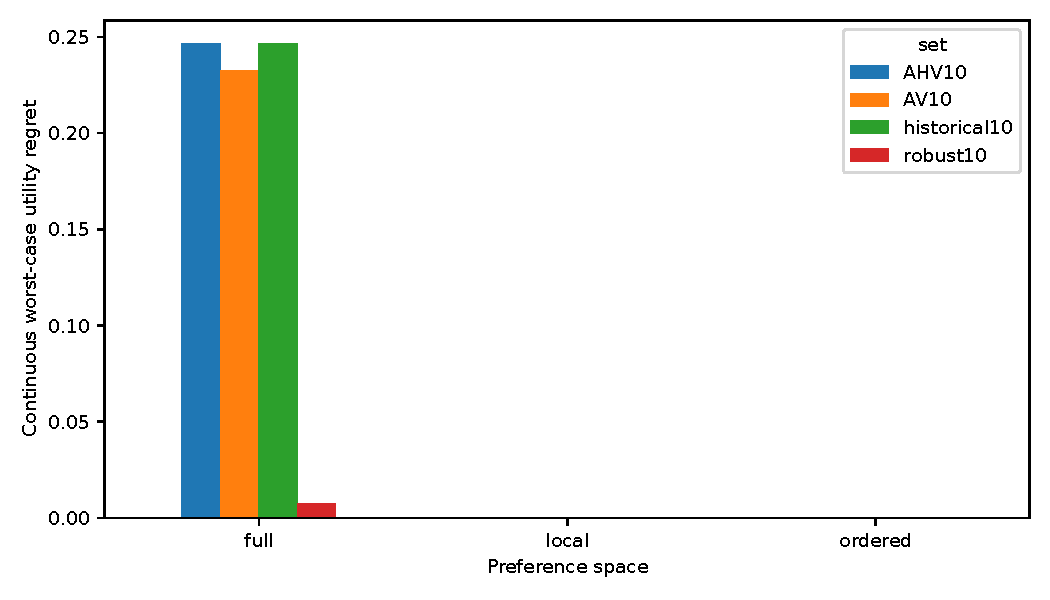
\includegraphics[width=\textwidth]{figures/continuous_regret.pdf}
\caption{Fixed-set continuous worst-case regret from the saved linear-programming audit. The full-simplex improvement does not imply a strict improvement in the two restricted spaces, where the compared sets already have zero regret.}\label{fig:continuous}
\end{figure}

\subsection{The Negative Result: Top-Ten Recovery Falls}
Opportunity preservation comes with a clear loss on a different outcome. Full-space top-ten recovery falls from 0.515600 for Historical10 to 0.422480 for Robust10. Under ordered weights it falls from 0.896180 to 0.443420, and under local weights from 0.899530 to 0.533730. The robust set is therefore not a more faithful approximation of every preference-specific top ten. It trades several near-centre high-ranked options for alternatives that protect other parts of preference space.

This finding is not a statistical anomaly to hide behind a small mean regret. If architects want several options close to their stated preferences, Historical10 can be more appropriate. If they have not agreed on priorities and want at least one strong option for a wide range of plausible weights, the regret objective is better aligned with that purpose. The study provides evidence for the second use, while retaining the first as a legitimate alternative. No human experiment establishes which service architects would prefer in practice.

\subsection{Continuous Audit, Replication and Sampling Error}
\begin{table}[tbp]\caption{Continuous fixed-set worst regret, with full-space grid maxima. All candidate-specific linear programs succeeded. Full fronts are unequal-budget references.}\label{tab:audit}\centering
\small
\begin{tabular}{lrrrrr}\toprule
Set & Size & Full LP & Full grid & Ordered LP & Local LP\\\midrule
historical10 & 10 & 0.246359 & 0.246359 & 0 & 0\\
AV10 & 10 & 0.232558 & 0.232558 & 0 & 0\\
AHV10 & 10 & 0.246359 & 0.246359 & 0 & 0\\
robust10 & 10 & 0.007656 & 0.007576 & 0 & 0\\
AV full & 12 & 0.232558 & 0.232558 & 0 & 0\\
AHV full & 41 & 0.000000 & 0.000000 & 0 & 0\\
\bottomrule\end{tabular}

\end{table}


The continuous audit in Table~\ref{tab:audit} confirms that the full-space historical maximum is 0.246359 at the pure-volume vertex $(0,0,1)$. Robust10's maximum is 0.007656, with an interior-edge witness approximately $(0.211837,0,0.788163)$ and competing candidate C13/C29. Checking only the three simplex vertices would miss this robust worst case. The grid maximum is 0.007576 and the test maximum is 0.007539, both below the continuous value as expected. The audit certifies the fixed-set loss within numerical tolerances; it does not certify a globally optimal ten-candidate set.

The unrestricted 41-member $A/H/V$ front has zero regret throughout all three continuous spaces. This is consistent with nonnegative linear utility: a dominated candidate cannot uniquely improve the maximum. Its 41 alternatives exceed the review budget, so this is an opportunity reference rather than a fair ten-candidate superiority claim. The unrestricted 12-member $A/V$ front still has full-space worst regret 0.232558 at pure duration preference; extra members cannot repair an omitted criterion.

Independent full-space replication gives mean regret 0.011351 for Historical10 and 0.000055 for Robust10, with winner coverage 0.76635 and 0.97885, respectively. The paired robust-minus-historical mean regret difference on the test split is $-0.010705$, with a conditional Monte Carlo 95\% interval $[-0.011132,-0.010279]$; replication gives $-0.011296$ and $[-0.011736,-0.010855]$. Ordered and local replication retain zero regret for both sets. Thus the prespecified criterion of no larger mean and 95th-percentile regret in every space, with a strict improvement somewhere, is met. This is improvement in the full space and equality in the other two, not strict improvement everywhere.


Across all 630 candidates, the largest absolute test--replication top-ten-acceptability difference is 0.01015 in the full space, 0.00725 in the ordered space and 0.00920 locally. The full-space maximum winner-acceptability difference is 0.00650; both restricted spaces have zero winner difference. These diagnostics support the broad qualitative pattern, not the significance of each last decimal. No simultaneous confidence claim or physical error bound follows from the sampling precision.

All ten greedy additions reduce the training maximum, from 0.341577 at the first candidate to 0.007269 at ten. It never reaches zero. The final set is not padded with slots after achieving perfect coverage. Nonetheless, individual greedy choices can be redundant in some preference regions, and no exchange-based or exact shortlist optimizer is compared. The measured improvement belongs to this frozen heuristic, training distribution and case, not to an optimality theorem.

\subsection{Actual Candidates and Evidence Status}
\begin{table}[tbp]\caption{Historical top ten in immutable score order. All have archived rule-level Honeybee review. C indicates a corrected translated design; U an unchanged contained result reused; -- missing translation.}\label{tab:historical}\centering
\small
\begin{tabular}{rlrrrrc}\toprule
Rank & Pair & $A$ (m$^2$) & $H$ (h) & $V$ (m$^3$) & $S$ & Trans.\\\midrule
1 & C9/C24 & 396 & 0.04874 & 5551.3 & 0.84486 & C\\
2 & C9/C15 & 351 & 0.03496 & 3127.8 & 0.75237 & C\\
3 & C9/C12 & 306 & 0.04357 & 4030.5 & 0.73582 & --\\
4 & C15/C24 & 243 & 0.05367 & 4016.5 & 0.72005 & --\\
5 & C9/C35 & 297 & 0.04481 & 5303.3 & 0.71420 & --\\
6 & C9/C13 & 333 & 0.03028 & 2975.2 & 0.70832 & U\\
7 & C12/C24 & 198 & 0.06228 & 4919.3 & 0.70350 & --\\
8 & C9/C21 & 333 & 0.03250 & 4252.0 & 0.70229 & --\\
9 & C9/C26 & 315 & 0.03520 & 3906.1 & 0.70170 & --\\
10 & C9/C27 & 324 & 0.03890 & 7340.9 & 0.68323 & --\\
\bottomrule\end{tabular}

\end{table}

\begin{table}[tbp]\caption{Robust10 in greedy addition order. HB denotes archived rule review (Y) or missing review (--); translation C means an archived contained correction and -- means missing verification. Historical rank is retained for comparison.}\label{tab:robust}\centering
\small
\begin{tabular}{rlrrrrcc}\toprule
Step & Pair & Hist. & $A$ & $H$ (h) & $V$ (m$^3$) & HB & Trans.\\\midrule
1 & C9/C12 & 3 & 306 & 0.04357 & 4030.5 & Y & --\\
2 & C12/C15 & 20 & 153 & 0.04850 & 2495.7 & -- & --\\
3 & C12/C24 & 7 & 198 & 0.06228 & 4919.3 & Y & --\\
4 & C9/C24 & 1 & 396 & 0.04874 & 5551.3 & Y & C\\
5 & C15/C25 & 125 & 99 & 0.02265 & 964.9 & -- & --\\
6 & C9/C15 & 2 & 351 & 0.03496 & 3127.8 & Y & C\\
7 & C25/C29 & 397 & 18 & 0.00320 & 387.4 & Y & --\\
8 & C13/C15 & 55 & 135 & 0.03520 & 1440.3 & Y & --\\
9 & C24/C35 & 11 & 189 & 0.06352 & 6192.0 & -- & --\\
10 & C15/C24 & 4 & 243 & 0.05367 & 4016.5 & Y & --\\
\bottomrule\end{tabular}

\end{table}



Tables~\ref{tab:historical} and \ref{tab:robust} retain actual pair identities and performances. Robust10 shares five candidates with Historical10: C9/C24, C9/C15, C9/C12, C15/C24 and C12/C24. It adds C12/C15, C15/C25, C25/C29, C13/C15 and C24/C35, and drops C9/C35, C9/C13, C9/C21, C9/C26 and C9/C27. The set Jaccard overlap is $5/15=1/3$. The greedy addition order in Table~\ref{tab:robust} is not a new fixed-weight ranking.

The added candidates have interpretable roles. C25/C29 offers only 18~m$^2$ of area benefit and 0.003200~h mean gain, but its nominal volume is 387.382~m$^3$, the universe minimum. C24/C35 gives 0.063516~h, the maximum mean gain, at 189~m$^2$ area reduction and 6,192.045~m$^3$ nominal volume. C12/C15 and C15/C25 provide intermediate combinations, while C13/C15 contributes a lower-volume alternative. Their inclusion reflects coverage of different utility directions, not a claim that smaller sunlight gains are generally preferable.

Seven Robust10 members have archived rule-level Honeybee results. Three do not: C12/C15, C15/C25 and C24/C35. All ten historical members have such review. The new shortlist thus expands the validation frontier rather than inheriting full review from its predecessor. Two robust members, C9/C24 and C9/C15, also have archived contained-translation corrections checked by Honeybee. Eight robust members lack archived translated-design verification. Missing evidence remains missing; high acceptability or a small regret is not a substitute.

\section{Integration with Simulation and Geometry Review}
\subsection{A Decision Workflow with Distinct Evidence Gates}
The intended workflow begins with an urban-block model, explicit eligibility and a fixed intervention rule.\aidraft{} Fast exposure evaluation produces the complete metric table. Preference analysis then produces rank distributions and alternative ten-candidate sets. The architect examines their trade-offs and review status before requesting additional simulation or developing geometry. Figure~\ref{fig:workflow} separates these activities.

\begin{figure}[tbp]\centering
\fbox{\begin{minipage}{0.91\textwidth}\centering
Canonical block and research eligibility\\[3pt]
$\downarrow$ 36 eligible groups; fixed two-building rule\\[3pt]
630 candidates with archived $A,H,V,N$\\[3pt]
$\downarrow$ Declared preference spaces and independent evaluation\\[3pt]
Rank acceptability $+$ Historical10 / Robust10 / Pareto alternatives\\[3pt]
$\downarrow$ Candidate-level evidence and unresolved constraints\\[3pt]
Selective rule simulation $\longrightarrow$ translated-solid checks\\[3pt]
$\downarrow$ Updated evidence, rights, structure and design judgment\\[3pt]
Architect decides which intervention to develop
\end{minipage}}
\caption{Proposed decision-support sequence. Simulation and geometry review are separate gates; the new preference experiment does not execute them or observe architects using the workflow.}\label{fig:workflow}\end{figure}

A practical first conversation is whether the full simplex is appropriate. If a project team rules out volume-dominant weights and accepts $w_A\geq w_H\geq w_V$, the result already establishes zero fixed-set regret for Historical10 over that continuous support. If priorities remain open, Robust10 retains more opportunities, but the team must budget for three previously unreviewed rule candidates and eight missing translations. If the objective is to offer multiple similar high-benefit options, top-ten recovery can be more relevant than winner coverage. The interface should expose these choices rather than display one unqualified ``best'' list.

Candidate rejection for ownership, structural or heritage reasons changes the feasible universe. Such exclusions cannot be treated as harmless after-the-fact annotations: the best available utility and regret benchmark can change. A revised analysis should record exclusions and recompute utilities and set evaluation against the revised feasible alternatives, with any normalization policy made explicit. The frozen experiment remains a reference, not an authorization to intervene in a building.

\subsection{Preserved Selective Simulation Evidence}
Historical evidence comprises 23 curated rule reviews and a disjoint, pre-frozen 20-candidate same-site coverage cohort. The curated pool combined historical top-ten, area--volume, historical and reference choices; it was purposive. The coverage cohort was selected for score strata, volume and identifier coverage before its reported Honeybee outcomes, rather than randomly across sites. Its identities and outcomes are not reselected in this work. There are 43 reviewed pairs, or about 6.83\% of the full universe, but agreement is reported by cohort.

\begin{table}[tbp]\caption{Historical same-metric comparison with archived Honeybee aggregates, preserved as supporting evidence. No new simulation is implied.}\label{tab:agreement}\centering
\begin{tabular}{llrrr}\toprule Cohort & Metric & Spearman $\rho$ & MAE & Exact\\\midrule
Curated23 & $A$ (m$^2$) & .999258 & .391304 & 22/23\\ & $H$ (h) & .991597 & .001177 & 3/23\\ & $S$ & .999012 & .006933 & 3/23\\
Coverage20 & $A$ (m$^2$) & .997668 & .450000 & 19/20\\ & $H$ (h) & .999624 & .000295 & 9/20\\ & $S$ & 1.000000 & .002139 & 9/20\\\bottomrule\end{tabular}\end{table}

Table~\ref{tab:agreement} compares like metrics, not score ranks against area ranks. Coverage-area MAE 0.45~m$^2$ arises from one 9~m$^2$ discrepancy among 20 candidates, not sub-grid accuracy. A score correlation of one is not exact score agreement; only nine coverage scores agree exactly. $V$ is shared between routes and $N$ is constant, further limiting independence of the composite comparison. Cohort overlap at a top-$K$ cutoff depends on tie handling and cannot establish full-universe recall.

The archived Honeybee/Ladybug effective rays differ from saved pvlib rays. WEA carriers use constant direct-normal irradiance 1000~W/m$^2$ and diffuse-horizontal irradiance zero; they encode direct-sun-hours calculations rather than measured meteorology. WEA and hour-of-year records do not carry a year field. Thus high aggregate agreement is evidence about these actual routes and settings, not an identical astronomical-input experiment or validation of annual environmental performance. No new raw site simulation is possible from the aggregate-only evidence used in the preference analysis.

\subsection{Historical Efficiency and Translation Failure}
The historical matched timing experiment compares repeated intersections with reusable building blockers under the same geometric primitive, rays and single-thread conditions. For selected pair $(a,b)$, if $O_{ijt}$ and $R_{ijt}$ are original and reduced-height blocker indicators, the count update is
\begin{equation}
 C_{jt}^{(a,b)}=C_{jt}-O_{ajt}-O_{bjt}+R_{ajt}+R_{bjt},\quad C_{jt}=\sum_i O_{ijt}.
\label{eq:blocker}
\end{equation}
Using an adequate signed integer type preserves the unchanged building contributions. Pointwise and aggregate equivalence passed in all 12 measured scale/repeat comparisons. At 630 candidates, medians from three repeats are 11,608.183~s for repeated intersections and 24.037~s for reuse, including preparation: a ratio of 482.927. This is a comparison of two implementations, without an indexed baseline, and is not a Honeybee speedup or a measurement of architects' work time.

Geometry translation remains a separate risk. Four of five archived translated pairs failed solid containment. In historical C9/C24 and C13/C24 translations, rays hit newly added upper walls outside the original footprint; each had four worsened receiving points and 9~m$^2$ of newly low-sun area. Controlled historical replays reproduced six scene visibility matrices, and four contained corrections were simulated separately. C9/C13 was already contained and reused its unchanged result. These are ten historical scene runs, not a new full-universe simulation.

The four corrections removed observed adverse visibility events on the fixed model, rays and receivers. For C9/C24, translated low-sun-area reduction changed from 342 to 351~m$^2$; the rule screening value is 396~m$^2$. Those values describe different objects and cannot be exchanged. C9/C15's translated area remained 342~m$^2$, while its rule value is 351~m$^2$. Correcting containment did not make the designs volume matched or equivalent to the original rules.

The distinction also affects costs. C9/C24 has nominal rule volume 5,551.333~m$^3$, rule-solid union reduction 5,470.406~m$^3$ and corrected translated union reduction 5,474.582~m$^3$. For C6/C33 these values are 5,583.055, 1,909.864 and 2,554.767~m$^3$. Overlaps and translated shape changes make these quantities materially different. Robustness of a utility based on nominal $V$ cannot establish robustness of a construction-cost decision based on another quantity.

\section{Discussion, Limitations and Reproducibility}
\subsection{What the New Evidence Supports}
The strongest contribution is a changed decision contract.\aidraft{} Historical fixed weights answer which candidates score highly under one priority statement. The new analysis asks how much choice is lost if only ten are retained before priorities are settled. Its full-space results show that five substitutions can preserve a much broader range of winning opportunities. The continuous audit further establishes that the improvement is not merely the failure of random sampling to encounter extreme weights.

The same evidence limits the claim. Restricted-space results show no need for a new set to preserve an optimal utility opportunity. The decline in top-ten recovery shows that the set is not universally more representative. A single candidate can secure zero regret for a region while other slots serve a different region, leaving few locally high-ranked alternatives. Therefore the contribution should be described as preference-robust opportunity screening under a specified objective, not a superior architectural recommendation list in every sense.

There is also a validation cost. The historical shortlist benefited from curated review, while three robust alternatives remain 2.5D-only. A workflow that quietly calls those alternatives validated would confuse preference analysis with physical evidence. Instead, the new shortlist tells the architect where further review is needed. Prioritizing those missing reviews would be a concrete next experiment, followed by re-evaluation if their performance values materially change. It cannot be replaced by attaching the old cohort's correlation to each new candidate.

\subsection{Threats to Validity}
\paragraph{Preference model.} Additive normalized utility assumes compensation between area, exposure and volume. Bounds and units shape its trade-offs. Uniform simplex area, the ordered restriction, local radius and equal-space mixture are research choices without architect elicitation. Correlated $A$ and $H$ may give sunlight improvement two related channels of influence. Other utility forms, vetoes or explicit removal budgets could change selection. The present results do not establish that any of these weights represent a target professional population.

\paragraph{Optimization and evaluation.} Greedy construction is path dependent and is not globally optimal. Historical-ranking compression makes AV10 and AHV10 useful transparent baselines but not strong optimized subset competitors. The study lacks a swap heuristic, exact combinatorial benchmark or broader budget search. The independent LP audit evaluates fixed sets on the chosen supports only. Monte Carlo confidence intervals describe sampling precision conditional on fixed performances; they do not cover model uncertainty, selection across many reported quantities or differences between sites.

\paragraph{Canonical geometry and solar scope.} Component-bounding-box unions are not verified as-built footprints. Shared components, overlaps and OBJ differences can affect both shade and volume. The single date, 16 time samples, 3~m receiver grid, 0.1~m height, assumed north and 3~h threshold delimit physical interpretation. Threshold crossings can be sensitive to small exposure changes. Neither annual performance, indoor daylight, glare, energy outcomes nor statutory compliance is established.

\paragraph{Evidence coverage.} Curated23 and coverage20 remain nonprobability same-site cohorts. Aggregate agreement can conceal spatial differences and cannot be transferred automatically to unreviewed alternatives. Archived rule and translated-design results concern different geometries. Containment removes the observed outside-footprint failure under tested conditions, but does not prove structural feasibility, equal removal cost or general correctness of arbitrary imported meshes. There is no new Honeybee experiment, architect survey, realized intervention or measured decision-time saving.

\paragraph{Scope of generalization.} All 630 alternatives share one rule family and a single canonical block. Exactly two altered groups excludes many plausible interventions. Property rights, function, heritage, construction sequencing and social impacts are outside the objective vector. A shortlist suitable for this early screening task may be unsuitable after those constraints are imposed. Replication weights test numerical sampling stability, not external validity.

\subsection{Reproducibility and Release Boundaries}
The new package retains a pre-outcome protocol and input hashes; scripts and software versions; every retained weight; all 630 rank histograms; candidate memberships; scenario-level test, replication and grid results; greedy traces; continuous LP status and witnesses; and tables linked to saved CSVs. Historical inputs and manuscripts remain unmodified. This enables re-execution of the preference analysis from fixed aggregate performances, including unfavorable outcomes.

The evidence distinguishes newly computed weight analysis, recomputed archived tables, historically measured timing, historical geometry replays and unchanged results reused for comparison. No newly computed utility is presented as a new physical observation. Missing rule review and missing translation are separate fields. The archive also preserves negative results rather than dropping candidate regions that reduce the strength of the narrative.

Raw CAD, DXF, SKP and OBJ inputs, receiver coordinates, Honeybee models, WEA carriers and Radiance intermediates remain restricted. The aggregate and algorithmic package does not confer permission to redistribute them or fully reproduce site simulations. Anonymous review materials exclude identifying repository links. Any broader release requires rights and anonymity review. These limitations reduce independent physical reproducibility even though the new preference experiment is reproducible from the retained table.

\section{Conclusion}
A fixed top ten cannot answer every screening question when priorities are unresolved.\aidraft{} For a finite universe of 630 solar-access height-reduction rules, we removed a constant risk metric from active weight discrimination, retained the historical score unchanged and evaluated three explicit preference spaces. A greedy sampled-minimax ten-candidate set substantially improves full-simplex opportunity preservation, with mean held-out regret 0.000054 and continuous worst-case regret 0.007656, compared with 0.010759 and 0.246359 for the historical set.

The result is conditional and informative in both directions. Historical10 already achieves zero regret under ordered solar-access-priority and local historical weights. Robust10 reduces top-ten membership recovery in all spaces and introduces three candidates without archived rule-level Honeybee review. These outcomes distinguish preserving a good eventual choice from reproducing a familiar ranking. They also identify concrete next work: eliciting actual project preferences, reviewing the newly exposed candidates and checking geometry before design commitments.

The contribution is an evidence-linked architectural decision-support application of established acceptability and regret concepts. It does not supply a new general algorithm, validated architect preferences or physical-model robustness. Fast enumeration, preference analysis, selective simulation and geometric checks become useful together when their outputs remain distinguishable and the final decision stays with the responsible professionals.

\section*{AI Use Disclosure}
An OpenAI assistant~\cite{openai2026} provided substantial assistance with the abstract and Sections~1--8: literature and evidence organization, experimental protocol and analysis-code preparation, numerical reporting, mathematical presentation, manuscript drafting and revision, tables, figure preparation and LaTeX quality checks. Section-specific citations identify assisted text. Charts and tables derive from saved experimental outputs; the workflow figure is a schematic, not site imagery. The assistant also supports accompanying translation. The exact underlying model version was not recorded. This disclosure does not assert completed independent author verification or approval. Authors must verify the scientific content, assistance scope and applicable declarations before submission.
\FloatBarrier
\bibliographystyle{splncs04}\bibliography{references}
\end{document}
